\chapter{Details on Natural Gradient Descent with CIQ-Based SVGP}
\label{app:ngd}

\section{$\mathcal{O}(M^2)$ Natural Gradient Updates}
\label{app:ngd}

When performing variational inference, we must optimize the $\bmm'$ and $\bS'$ parameters of the whitened variational distribution $q(\bu') = \normaldist{\bmm'}{\bS'}$.
Rather than using standard gradient descent methods on these parameters, many have suggested that {\bf natural gradient descent (NGD)} methods are better suited for variational inference \cite{hoffman2013stochastic,hensman2012fast,salimbeni2018natural}.
NGD performs the following update:
%
\begin{equation}
  \begin{bmatrix} \bmm & \bS \end{bmatrix} \gets \begin{bmatrix} \bmm & \bS \end{bmatrix} - \varphi  \bFS^{-1}
  \begin{bmatrix} \frac{\partial \text{ELBO}}{\partial \bmm} & \frac{\partial \text{ELBO}}{\partial \bS} \end{bmatrix}
\end{equation}
%
where $\varphi$ is a step size, $\begin{bmatrix} \frac{\partial \text{ELBO}}{\partial \bmm} & \frac{\partial \text{ELBO}}{\partial \bS} \end{bmatrix}$ is the ELBO gradient, and $\bFS$ is the \emph{Fischer information matrix} of the variational parameters.
Conditioning the gradient with $\bFS^{-1}$ results in descent directions that are better suited towards distributional parameters \cite{hoffman2013stochastic}.

For Gaussian distributions (and other exponential family distributions) the Fischer information matrix does not need to be explicitly computed.
Instead, there is a simple closed-form update that relies on different parameterizations of Gaussian distributions.
%
\begin{equation}
  \begin{bmatrix} \btheta & \bTheta \end{bmatrix} \gets \begin{bmatrix} \btheta & \bTheta \end{bmatrix} - \varphi
  \begin{bmatrix} \frac{\partial \text{ELBO}}{\partial \boeta} & \frac{\partial \text{ELBO}}{\partial \bEta} \end{bmatrix}.
\end{equation}
%
$[\btheta, \:\: \bTheta]$ are the Gaussian's \emph{natural parameters}
and $[\boeta, \:\: \bEta]$ are the Gaussian's \emph{expectation parameters}:
%
\begin{align*}
  \btheta = \bS^{-1} \bmm, &\quad
  \bTheta = -\frac 1 2 \bS^{-1}, \\
  \boeta = \bmm, &\quad
  \bEta = \bmm \bmm^\top + \bS
\end{align*}

In many implementations, it is common to store the variational parameters via their natural representation ($\btheta$, $\bTheta$), compute the ELBO via the standard parameters ($\bmm'$, $\bS'$), and then compute the derivative via the expectation parameters ($\boeta$, $\bEta$).
Unfortunately, converting between these three parameterizations requires $\bigo{M^3}$ computation.
(To easily see why this is the case, note that computing $\bS'$ essentially requires inverting the $\bTheta$ matrix.)

\paragraph{A $\bigo{M^2}$ NGD update.}
In what follows, we will demonstrate that the ELBO and its derivative can be computed from $\btheta$ and $\bTheta$ in $\bigo{M^2}$ time via careful bookkeeping.
Consequentially, for NGD updates have the same asymptotic complexity as the other computations required for SVGP.
Recall that the ELBO is given by
\[
  \text{ELBO} = \overbracket{ \sum_{i=1}^N \Evover{q(f(\bx^{(i)}))}{  \: \log p( y^{(i)} \mid f(\bx^{(i)}) ) \: }}^{\text{expected log likelihood}} - \kl{ q(\bu) }{ p(\bu) }
\]
We will analyze the computations for the expected log likelihod term and the KL divergence term separately.

\subsection{The Expected Log Likelihood and its Gradient}
Assume we are estimating the ELBO from a single data point $\bx, y$.
The expected log likelihood term of the ELBO is typically computed via quadrature or Monte Carlo integration \cite{hensman2015scalable}:\footnote{
  It can also be computed analytically for Gaussian distributions \cite{hensman2013gaussian}.
  The analytic form achieves the same derivative decomposition as in \cref{eqn:ell_deriv_decomp}
  and so the following analysis will still apply.
}
%
\[
  \Evover{q(f(\bx)}{ \log p(y \mid f(\bx)) } = \sum_{s=1}^S w_s p(y \mid f_s),
  \quad
  f_s = \ameantest{\bx} + \avartest{\bx}^{1/2} \varepsilon_s
\]
%
where $w_s$ are the quadrature weights (or $1/S$ for MC integration) and $\varepsilon_s$ are the quadrature locations (or samples from $\normaldist{0}{1}$ for MC integration).
Therefore, the variational parameters only interact with the expected log likelihood term via $\ameantest{\bx}$ and $\avartest{\bx}$.
We can write its gradients via chain rule as:
%
\begin{align}
  \frac{ \partial \Evover{q(f(\bx)}{ \log p(y | f(\bx)) }}{\partial \boeta}
  \:\: &= \:\:
  c_1 \: \frac{ \partial \ameantest{\bx}}{\partial \boeta}
  \:\: + \:\:
  c_2 \:  \frac{ \partial \avartest{\bx}}{\partial \boeta}
  \nonumber \\
  \frac{ \partial \Evover{q(f(\bx)}{ \log p(y | f(\bx)) }}{\partial \bEta}
  &=
  c_3 \: \frac{ \partial \ameantest{\bx}}{\partial \bEta}
  \:\: + \:\:
  c_4 \:  \frac{ \partial \avartest{\bx}}{\partial \bEta}
  \label{eqn:ell_deriv_decomp}
\end{align}
%
for some constants $c_1$, $c_2$, $c_3$, and $c_4$ that do not depend on the variational parameters.
It thus suffices to show that the predictive mean/variance and their gradients can be computed from $\btheta$ and $\bTheta$ in $\bigo{M^2}$ time.

\paragraph{The predictive distribution and its gradient.}
All expensive computations involving $\btheta$ and $\bTheta$ are written in {\color{blue} blue}.

$\ameantest{\bx}$ and its derivative can be written as:
%
\begin{align}
  \ameantest{\bx}
  &= \bk_{\bZ \bx}^\top \bK_{\bZ\bZ}^{-1/2} \bmm'
  \tag{standard parameters} \\
  &= \bk_{\bZ \bx}^\top \bK_{\bZ\bZ}^{-1/2} \boeta
  \tag{expectation parameters} \\
  &= {\color{blue} \bk_{\bZ \bx}^\top \bK_{\bZ\bZ}^{-1/2} (-2 \bTheta)^{-1}} \btheta
  \label{eqn:pred_mean_natural},
  \\
  \frac{\partial \ameantest{\bx}}{\partial \boeta}
  &= \bK_{\bZ\bZ}^{-1/2} \bk_{\bZ \bx}
  \label{eqn:pred_mean_deriv},
  \\
  \frac{\partial \ameantest{\bx}}{\partial \bEta}
  &= \bzero.
  \nonumber
\end{align}

$\avartest{\bx}$ and its derivative can be written as:
%
\begin{align}
  \avartest{\bx}
  &= \bk_{\bZ \bx}^\top \bK_{\bZ\bZ}^{-1/2} \left( \bS' - \bI \right) \bK_{\bZ\bZ}^{-1/2} \bk_{\bZ \bx}
  \tag{standard parameters} \\
  &= \bk_{\bZ \bx}^\top \bK_{\bZ\bZ}^{-1/2} \left( \bEta - \boeta \boeta^\top - \bI \right) \bK_{\bZ\bZ}^{-1/2} \bk_{\bZ \bx}
  \tag{expectation parameters} \\
  &= {\color{blue} \bk_{\bZ \bx}^\top \bK_{\bZ\bZ}^{-1/2} \left((-2 \bTheta)^{-1} \right.} \left. - \bI \right) \bK_{\bZ\bZ}^{-1/2} \bk_{\bZ \bx}
  \label{eqn:pred_var_natural},
  \\
  \frac{\partial \avartest{\bx}}{\partial \boeta}
  &= {\color{blue} \bk_{\bZ \bx}^\top \bK_{\bZ\bZ}^{-1/2} (-2 \bTheta)^{-1}} \btheta
  \label{eqn:pred_var_deriv_1},
  \\
  \frac{\partial \avartest{\bx}}{\partial \bEta}
  &= \left( \bK_{\bZ\bZ}^{-1/2} \bk_{\bZ \bx}^\top \right) \left( \bk_{\bZ \bx}^\top \bK_{\bZ\bZ}^{-1/2} \right)
  \label{eqn:pred_var_deriv_2}.
\end{align}
%
In \cref{eqn:pred_mean_natural,eqn:pred_mean_deriv,eqn:pred_var_natural,eqn:pred_var_deriv_1,eqn:pred_var_deriv_2}, the only expensive operation involving $\bK_{\bZ\bZ}$ is $\bK_{\bZ\bZ}^{-1/2} \bk_{\bZ \bx}$, which can be computed with CIQ.
The only expensive operation involving the variational parameters is ${\color{blue} (-2 \bTheta)^{-1} \bK_{\bZ\bZ}^{-1/2} \bk_{\bZ \bx}}$, which can be computed with preconditioned conjugate gradients after computing $\bK_{\bZ\bZ}^{-1/2} \bk_{\bZ \bx}$.\footnote{
  We typically apply a Jacobi preconditioner to these solves.
}
Those operations only need to be computed once, and then they can be reused across \cref{eqn:pred_mean_natural,eqn:pred_mean_deriv,eqn:pred_var_natural,eqn:pred_var_deriv_1,eqn:pred_var_deriv_2}.
In total, the entire computation for the expected log likelihood and its derivative is $\bigo{M^2}$.

\subsection{The KL Divergence and its Gradient}
We will demonstrate that the KL divergence and its gradient can be computed from $\btheta$ and $\bTheta$ in $\bigo{M^2}$ time.
All expensive computations involving $\btheta$ and $\bTheta$ are written in {\color{blue} blue}.

The whitened KL divergence from \cref{sec:variational_results} can be re-written as:
%
\begin{align}
  \kl{ q(\bu') }{ p(\bu') }
  &= \frac{1}{2} \left[ \bmm^{\prime \top} \bmm' + \tr{ \bS' } - \log \vert \bS' \vert - M \right]
  \tag{standard parameters} \\
  &= \frac{1}{2} \left[ \tr{ \bEta } - \log \vert \bEta - \boeta \boeta^\top \vert - M \right]
  \tag{expectation parameters} \\
  &= \frac{1}{2} \left[ \btheta^\top {\color{blue} (-2 \bTheta)^{-2} \btheta} + {\color{blue} \tr{(-2 \bTheta)^{-1}}} + {\color{blue} \log \vert -2 \bTheta \vert} - M \right]
  \label{eqn:kl_natural}.
\end{align}
%
The KL derivative with respect to $\boeta$ and $\bEta$ is surprisingly simple when re-written in terms of the natural parameters
%
\begin{align}
  \frac{\partial \kl{ q(\bu') }{ p(\bu') }}{ \partial \boeta }
  &= \left( \bEta - \boeta \boeta^\top \right)^{-1} \boeta
  = (\bS')^{-1} \boeta
  \nonumber \\
  &= \btheta
  \label{eqn:kl_mean_deriv}
  \\
  \frac{\partial \kl{ q(\bu') }{ p(\bu') }}{ \partial \bEta }
  &= \frac 1 2 \bI - \frac 1 2 \left( \bEta - \boeta \boeta^\top \right)^{-1}
  = \frac 1 2 \bI - \frac 1 2 (\bS')^{-1} \boeta
  \nonumber \\
  &= \frac 1 2 \bI - \bTheta.
  \label{eqn:kl_covar_deriv}
\end{align}
%
Thus the derivative of the KL divergence only takes $\bigo{M^2}$ time to compute.
The forward pass can also be computed in $\bigo{M^2}$ time---using stochastic trace estimation for the trace term \citep{cutajar2016preconditioning,gardner2018gpytorch}, stochastic Lanczos quadrature for the log determinant \citep{ubaru2017fast,dong2017scalable}, and CG for the solves.
However, during training the forward pass can be omitted as only the gradient is needed for NGD steps.







\section{Additional SVGP Results}

\begin{figure}[ht!]
  \centering
  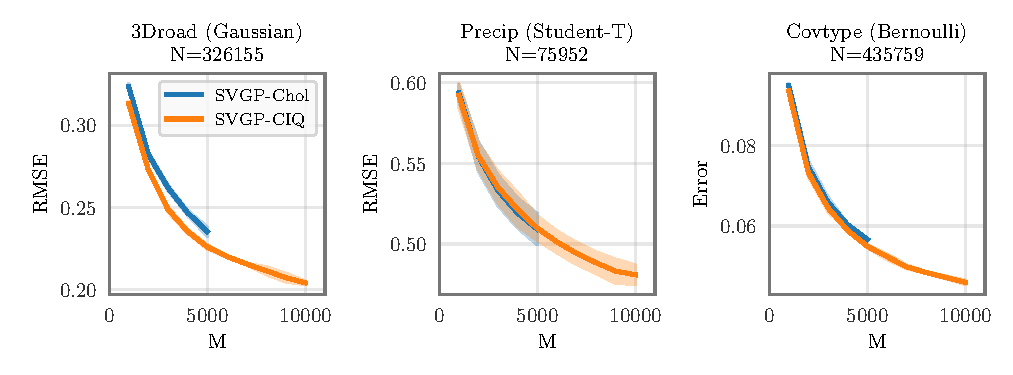
\includegraphics[width=\linewidth]{figures/variational_error.pdf}
  \caption[RMSE comparison of Cholesky-whitened vs CIQ-whitened SVGP models.]{
    RMSE comparison of Cholesky-whitened vs CIQ-whitened SVGP models.
    {\bf Left:} 3DRoad dataset ($N=326155, D=2$, Gaussian likelihood).
    {\bf Middle:} Precipitation dataset ($N=75952, D=3$, Student-T likelihood).
    {\bf Right:} CoverType dataset ($N=435759, D=54$, Bernoulli likelihood).
    NLL improves with more inducing points ($M$), and Cholesky and CIQ models have similar performance.
    However CIQ scales to larger values of $M$.
  }
  \label{fig:variational_error}
\end{figure}

In \cref{fig:variational_error} we plot the predictive error of CIQ-SVGP and Chol-SVGP models as a function of $M$.
For the two regression datasets (3droad and Precipitation) error is measured by test set root mean squared error (RMSE).
On the Covtype classification dataset error is measured by the $0-1$ loss on the test set.
As with the NLL results in \cref{fig:variational_nll} we find that the CIQ-SVGP and Chol-SVGP perform similarly, despite the fact that CIQ-SVGP can be up to $4\times$ faster.
Moreover, we see that error continuously decreases with more inducing points up to $M=10,\!000$.
